\documentclass[twoside,10pt]{article}
\usepackage{shlists}
\usepackage[applemac]{inputenc}
\usepackage[spanish]{babel}
\usepackage[T1]{fontenc}


\usepackage{multicol}
\usepackage{picinpar}

\usepackage{url}
\newcommand{\surl}[1]{{\small\url{#1}}}

\newcounter{vol}
\newcounter{num}
\newcounter{anyo}
\setcounter{vol}{9}
\setcounter{num}{2}
\setcounter{anyo}{2016}
\newcommand{\mes}{Mayo}
\usepackage{revisionNLcol}


\title{\ \\ Docencia 2.0\\ \large Juan Juli\'an Merelo, Fernando Tricas}
\author{\LARGE En defensa de los trabajos de fin de grado}

\date{}

\AutTit{Docencia 2.0}

\begin{document}
\addtocounter{page}{2}

\maketitle
\vspace*{-2ex}

\begin{multicols}{2}
 
Recientemente, con la transformaci\'on de los t\'itulos universitarios con
la convergencia al espacio europeo de educaci\'on superior se est\'an
escuchando cr\'iticas a la necesidad de realizar trabajos de fin de
Grado y M\'aster (TFG/TFM). Sobre todo en titulaciones donde no exist\'ia la
costumbre y se est\'an enfrentando a las complejidades del dise\~no de este
tipo de asignaturas. Simult\'aneamente, en las comisiones de acreditaci\'on se
pide que se incluya la nota obtenida por los alumnos a los que se les ha
dirigido tal trabajo, convirti\'endolos {\bf para algunos?}, de esa forma, en
una manera m\'as de evaluar al docente. 
% Yo creo que no deberíamos decir eso. Si acaso para algunos, o como un efecto
% pernicioso, no me gusta mucho. Pongo en negrita mi sugerencia

Queremos dedicar estas l\'ineas a las ventajas que vemos a este tipo de
trabajo que culminan unos estudios y que deber\'ian verse, por muchos
motivos, como un paso importante en vez de una molestia innecesaria
e inevitable, todo ello desde la experiencia de llevar unos cuantos
a\~nos impartiendo docencia en titulaciones de ingenier\'ia, donde el
proyecto de fin de carrera y luego los TFG/TFM son una
costumbre establecida. Aportamos la experiencia de haber dirigido unos cuantos
de estos trabajos y formado parte de otro buen n\'umero de tribunales
evaluadores. Del viejo, el consejo. Y de unas personas que ha estado en m\'as
tribunales de trabajos que Eva Hache en los de Got Talent, una serie de
valoraciones sobre los mismos. 

En el principio, eran las {\em tesinas}. Un trabajo, extenso,
posiblemente m\'as acad\'emico que otra cosa, que se presentaba con
chaqueta y corbata ante un serio tribunal de la c\'atedra m\'as pr\'oxima a
la carrera. En las ingenier\'ias, las tesinas devinieron
proyectos. %¿Esto es cierto? ¿Ese es el origen?
% Las ingenier\'ias siempre han tenido proyectos, pero cuando las
% licenciaturas eran en ingenier\'ia se les llam\'o proyectos - JJ
 Y los proyectos, eventualmente, se convirtieron en trabajos,
 perdiendo ese aura vital de algo que se emprende, que avanza. Un
 trabajo es algo que hay que entregar, pero que puede tener o no que
 ver con tu vida, o tu trabajo, {\em real}. 

A\'un as\'i, con su extensi\'on a muchos grados, un trabajo fin de grado o
TFG es algo que est\'a m\'as relacionado con la madurez del alumno que con
sus conocimientos t\'ecnicos; es transversal en el sentido que tiene que
servir no tanto para adquirir conocimientos t\'ecnicos, sino para ponerlos
en pr\'actica en una situaci\'on tan del mundo real como el tutor y el
alumno puedan permitirse.  Por eso, desde el punto de vista del
alumno y siguiendo el adagio ``Del viejo, el consejo'', convendr\'ia
tener en cuenta las siguientes ideas

Todos tenemos m\'ultiples facetas en la vida. 
`Party hard, work hard'. Seguro que nuestros allegados ya tienen claro que nos
defendemos con mayor o menor acierto cuando toca divertirse. El trabajo de fin
de estudios debe (o al menos puede) ser un trabajo que re\'una una parte
considerable de los conocimientos alcanzados en los estudios. Tambi\'en debe (o
puede) permitirnos explorar algunos temas laterales que no se hayan tratado de
manera completa en lo estudios regulares, o temas novedosos con cierto `riesgo'
que no sabemos si llegar\'an a alcanzar la consolidaci\'on dentro de la
disciplina. Las ense\~nanzas regladas son eso, regladas. En estos trabajos  se
  invita al alumno que se salte un poco las reglas. 

%--------------------------
\noindent\rule{86mm}{1pt}
\vspace{1ex} {\small{\begin{window}[0,r,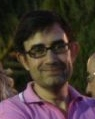
\includegraphics[width = 27
mm]{JJM.jpg},] \noindent\emph{JJ Merelo} es catedr\'{a}tico de Universidad
en el \'area de Arquitectura y Tecnolog\'{\i}a de Computadores, y
actualmente director de la Oficina de Software Libre de la UGR.
Mantiene un blog desde el a\~no 2002, y lo ha utilizado en clase desde
el a\~no 2004; tambi\'en wikis y, ultimamente, agregadores y otras
herramientas TIC. \'{U}ltimamente le ha dado por el \textsl{flipped
learning}, de lo que se informar\'{a} debidamente en esta columna.
\end{window}}}

\medskip

{\small{\begin{window}[0,r,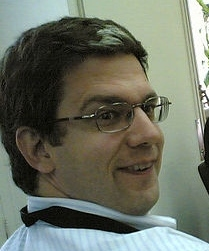
\includegraphics[width = 27 mm]{FTricas1.jpg},]
		\noindent  \emph{Fernando Tricas Garc\'{\i}a} es profesor
		titular de Lenguajes y Sistemas Inform\'aticos del Departamento
		de Inform\'atica e Ingenier\'{\i}a de Sistemas de la Universidad de
		Zaragoza.  Empez\'o a estudiar la blogosfera casi cuando a\'un no
		exist\'{\i}a (all\'a por el a\~no 2002) y a tratar de integrarla en los
		cursos y tareas docentes un poco despu\'es.  Ha impartido
		numerosas charlas relacionadas con el tema de la Web 2.0, internet y universidad, ...
		Es actualmente Vicerrector de Tecnolog\'ias de la Informaci\'on y
de la Comunicaci\'on.  
		\end{window}}}
%-------------------------------------------------

\noindent `If you can dream it, you can do it'. Salvo que tengamos un
  marcado esp\'iritu emprendedor el trabajo de fin de estudios puede ser
  una de las \'ultimas veces en las que podamos tomar nuestras propias
  decisiones sobre lo que queremos trabajar. Luego iremos a trabajar
  en el `mundo real'\textregistered\     y all\'i pasaremos una temporada
  haciendo lo que seguramente decidir\'an otros. En un proyecto, t\'u eres
  literalmente el jefe de proyecto, el responsable del mismo. La
  experiencia que tengas dirigi\'endote a ti mismo te puede ser \'util si,
  m\'as adelante, tienes que dirigir a alguien. 

`Yes we can'. Despu\'es de unos cuantos a\~nos estudiando podremos
  demostrar (y demostrarnos) que somos capaces de abordar un proyecto
  m\'as o menos grande (no tan grande, en realidad) pasando por diversos
  procesos que hemos aprendido en nuestros estudios: investigar,
  analizar, examinar alternativas, tomar decisiones y asumir sus
  consecuencias. S\'i, podemos, pero tambi\'en podemos equivocarnos y una
  refactorizaci\'on a un mes de la entrega te puede ense\~nar tanto como
  varias asignaturas de ingenier\'ia del software juntas. 

`Show me the money'. Tambi\'en somos defensores de la presentaci\'on del
  trabajo en sesi\'on p\'ublica y la liberaci\'on del mismo en un
  repositorio tal como GitHub. Seguramente hemos hecho presentaciones en
  algunas asignaturas, incluso de nuestro propio trabajo. Pero ahora
  vamos a presentar ante el p\'ublico y ante el tribunal (-qu\'e mala cara
  pon\'ia ese se\~nor que estaba segundo por la izquierda cuando dijiste
  eso-, podr\'a decir nuestra Tita Eduvigis que se puso las mejores
  galas para este gran momento, -yo creo que no han comprendido lo que
  quer\'ia decir- podr\'a explicar nuestro padre ante la insistencia del
  tribunal por aclarar determinada cuesti\'on) nuestro trabajo de varios
  meses: esas decisiones, dudas, tiempo invertido. Con suerte, en
  presencia de familiares y amistades que sentir\'an con nosotros la
  presi\'on del momento. Y la satisfacci\'on del resultado. 

`We did it'. Tampoco es despreciable el valor publicitario del
  proceso: un tribunal impresiona. M\'as a\'un a los for\'aneos que no saben
  que aquel d\'ia ten\'iamos unas cuantas horas de clase, la entrega de
  alguna revisi\'on y una evaluaci\'on de alguno de nuestros propios
  trabajos. As\'i que all\'i estamos mostrando a la sociedad que nos
  tomamos en serio el trabajo de los estudiantes, que hacen cosas que
  nos pueden resultar interesantes y \'utiles (e incluso, en algunos
  casos, de las que parecen saber m\'as que nosotros). Y, si lo has
  liberado, es algo que podr\'as mostrar a tus futuros inversores o
  empleadores. ``Lo hicimos'' y aqu\'i queda para la posteridad. 

`So proud of us'. En la mayor\'ia de los trabajos de fin de
  estudios el resultado es positivo, muchas veces por puro pundonor se
  retrasa la entrega hasta que sale todo como se desea. Pero, cuando
  se entrega, llega el momento de felicitarnos,
  que nos feliciten y sentirnos orgullosos de pertenecer a la lista de
  titulados de nuestro centro.


En definitiva, nos habremos enfrentado por primera vez a la toma de decisiones, asumir sus consecuencias, discutir sobre las mismas (primero con nuestro tutor y luego, tal vez con el tribunal) y mostrarlas ante un p\'ublico (m\'as o menos) entregado. Mostrando (y mostr\'andonos) que la carrera nos ha ayudado en el proceso de convertirnos en profesionales.

Por eso animamos a los que hayan perdido la fe en estos trabajos y a los que a\'un no la tienen para que aprecien y comprendan los posibles beneficios que puede tener este esfuerzo.
\bigskip

\noindent\emph{Todas las columnas de la serie Docencia 2.0
pueden descargarse en formato LaTeX desde
\surl{https://github.com/ReVision-Docencia-20/Columnas}}

\noindent\rule{90mm}{1pt}

{\small \noindent\copyright 2016 JJ. Merelo, F. Tricas. Este art\'{\i}culo es de acceso libre distribuido bajo los t\'erminos
de la Licencia Creative Commons de Atribuci\'on, que permite copiar,
distribuir y comunicar p\'ublicamente la obra en cualquier medio, s\'olido
o electr\'onico, siempre que se acrediten a los autores y fuentes
originales}

\end{multicols}
\end{document}
